\documentclass[a4paper,12pt]{report}
\addtolength{\oddsidemargin}{-1.cm}
\addtolength{\textwidth}{2cm}
\addtolength{\topmargin}{-2cm}
\addtolength{\textheight}{3.5cm}
\newcommand{\HRule}{\rule{\linewidth}{0.5mm}}
\makeindex

\usepackage{longtable}
\usepackage{graphicx}
\usepackage{makeidx}
\usepackage{hyperref}
\usepackage{verbatim}

\hypersetup{
    colorlinks=true,
    linkcolor=blue,
    filecolor=magenta,      
    urlcolor=cyan,
}


% define the title
\author{Ambitious Design}
\title{ Software Requirements Specifications and Technology Neutral Process Design}
\begin{document}
\setlength{\parskip}{6pt}

% generates the title
\begin{titlepage}

\begin{center}
% Upper part of the page           
\textsc{\LARGE Department of Computer Science}\\[1.5cm]
\textsc{\Large COS 301 - Main Project}\\[0.5cm]
% Title
\HRule \\[0.4cm]
{ \huge \bfseries Document 1}\\[0.4cm]
\HRule \\[0.4cm]
% Author and supervisor
\begin{minipage}{0.4\textwidth}
\begin{flushleft} \large
\emph{Author:}\\
Tim {Kirker}
\end{flushleft}
\end{minipage}
\begin{minipage}{0.4\textwidth}
\begin{flushright} \large
\emph{Student number:} \\
u11152402
\end{flushright}
\end{minipage}
\begin{minipage}{0.4\textwidth}
\begin{flushleft} \large
\emph{} \\
Stephen {Swanepoel}
\end{flushleft}
\end{minipage}
\begin{minipage}{0.4\textwidth}
\begin{flushright} \large
\emph{} \\
u11032091
\end{flushright}
\end{minipage}
\begin{minipage}{0.4\textwidth}
\begin{flushleft} \large
Dian {Veldsman}
\end{flushleft}
\end{minipage}
\begin{minipage}{0.4\textwidth}
\begin{flushright} \large
\emph{} \\
u12081095
\end{flushright}
\end{minipage}
\begin{minipage}{0.4\textwidth}
\begin{flushleft} \large
Killian {Kieck}
\end{flushleft}
\end{minipage}
\begin{minipage}{0.4\textwidth}
\begin{flushright} \large
\emph{} \\
u12252213
\end{flushright}
\end{minipage}


{\large \today}
\end{center}
\end{titlepage}
\footnotesize
\normalsize

\renewcommand{\thesection}{\arabic{section}}
\newpage
\begin{center}
\textsc{\LARGE Software Requirements Specification}\\[1.5cm]
\end{center}



\section{Introduction}

 \subsubsection{Vision}
 
\subsubsection{Background}
	
\section{Architecture Requirements}
\subsection{Access Channel Requirements}

\subsection{Quality Requirements}
\subsubsection{Performance}

\subsubsection{Reliability}


\subsubsection{Scalability}

\subsubsection{Security}

\subsubsection{Flexibility}

\subsubsection{Maintainability}

\subsubsection{Auditability}

\subsubsection{Integrability}

\subsubsection{Cost}

\subsubsection{Usability}
\newpage
 \subsubsection{Integration Requirements}
 The following are the integration requirements for the Smart Image Identifier project:
 	\begin{itemize}
 		\item Integration channels The main integration channel that will be used for this project is Javascipt. This will allow us to communicate with their temporary server that contains all the images we will be using for the project.
 	\end{itemize}
	\begin{itemize}
 		\item Protocols
	\end{itemize}
	\begin{itemize}
 		\item API specifications
	\end{itemize}
	\begin{itemize}
 		\item Quality requirements
			\begin{itemize}
				\item Performance: The performance for the integration is important, such that the sooner a human is identified the sooner measures can be taken. How ever we are limited to the speed of the camera transmitters and thus will focus on notifying the client as fast as we can as opposed to sending the image.
				\item Scalability: The clients will maintain their image servers so that they may take and store as many images as necessary. The application that will be used by the customers will be available through the app store and will allow for a large customer base to download it.
				\item Security: The clients picture servers must be completely secure as they contain incredibly sensitive data.
			\end{itemize}
	\end{itemize}
	
 \subsubsection{Architecture Constraints}
	Technologies to be used:
		\begin{itemize}
			\item OpenCv
			\\
		\end{itemize}
\newpage
\section{Functional Requirements and Application Design}
\subsection{Use Case Prioritisation}
	\begin{itemize}
		\item[$\bullet$]\textbf{Set Search Target}\newline

		\textbf{Description:} A person with access to software can set the what the smart image identifier must search for.\newline
		
		\textbf{Use Case Prioritisation:} Nice-To-Have\newline

		\textbf{Pre-Conditions:}
		\begin{itemize}
			\item[$\bullet$]Administrator must enter valid criteria to search for.
			\\
		\end{itemize}
		\textbf{Post-Conditions: }
		\begin{itemize}
			\item[$\bullet$]Administrator can see what the Smart Image Identifier is searching for.
			\\
		\end{itemize}
		\item[$\bullet$]\textbf{Create Table}\newline

		\textbf{Description:} Create new tables in the database to categorize the data into baskets.\newline
		
		\textbf{Use Case Prioritisation:} Critical\newline
		
		\textbf{Pre-Conditions:}
		\begin{itemize}
			\item[$\bullet$]System must have access to the database.
			\\
		\end{itemize}
		\textbf{Post-Conditions: }
		\begin{itemize}
			\item[$\bullet$]New database table is created.
			\\
		\end{itemize}
		\newpage
		\item[$\bullet$]\textbf{Insert Data}\newline

		\textbf{Description:} Move images (data) in the database from one table to another.\newline
		
		\textbf{Use Case Prioritisation:} Critical\newline

		\textbf{Pre-Conditions:}
		\begin{itemize}
			\item[$\bullet$]System must have access to the database.
			\item[$\bullet$]Table must exist.
			\\
		\end{itemize}
		\textbf{Post-Conditions: }
		\begin{itemize}
			\item[$\bullet$]Image is moved to selected table.
			\\
		\end{itemize}
		\item[$\bullet$]\textbf{Retrieve Data}\newline

		\textbf{Description:} Retrieve images (data) from the database to be analyzed.\newline
		
		\textbf{Use Case Prioritisation:} Critical\newline

		\textbf{Pre-Conditions:}
		\begin{itemize}
			\item[$\bullet$]System must have access to the database.
			\item[$\bullet$]Image(data) being retrieved must be in the database.
			\\
		\end{itemize}
		\textbf{Post-Conditions: }
		\begin{itemize}
			\item[$\bullet$]Image(data) is still inside the database.
			\\
		\end{itemize}
		\newpage
		\item[$\bullet$]\textbf{Delete Data}\newline

		\textbf{Description:} Removes images (data) from the database.\newline
		
		\textbf{Use Case Prioritisation:} Important\newline

		\textbf{Pre-Conditions:}
		\begin{itemize}
			\item[$\bullet$]System must have access to the database.
			\item[$\bullet$]Image(data) to be deleted must be in the database.
			\\
		\end{itemize}
		\textbf{Post-Conditions: }
		\begin{itemize}
			\item[$\bullet$]Image(data) is removed from the database.
			\\
		\end{itemize}
		\item[$\bullet$]\textbf{Alert}\newline

		\textbf{Description:} Alert the user when an image being searched contains the search criteria in it.\newline
		
		\textbf{Use Case Prioritisation:} Critical\newline

		\textbf{Pre-Conditions:}
		\begin{itemize}
			\item[$\bullet$]Image(data) must contain the search criteria in it.
			\\
		\end{itemize}
		\textbf{Post-Conditions: }
		\begin{itemize}
			\item[$\bullet$]User is alerted.
			\item[$\bullet$]Image(data) is included with the alert.
			\\
		\end{itemize}
	\end{itemize}
\subsection{Use Case/Services Contracts}
	\subsubsection{Smart Image Identifier Use Case}
	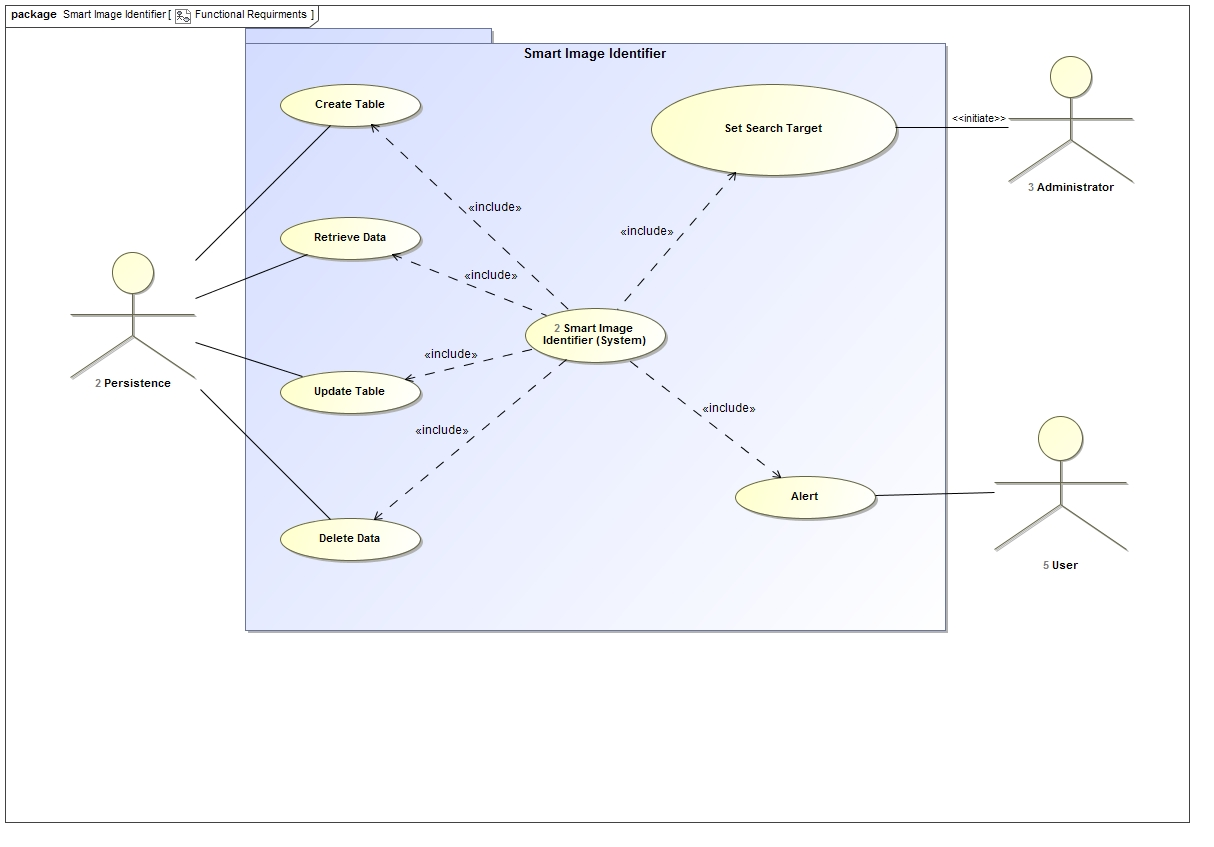
\includegraphics[width=1\textwidth]{./FunctionalRequirments.jpg}\\[1.5cm]
\end{document}